%! TEX root = ../main.tex
\documentclass[../main]{subfiles}

\begin{document}
\section{\texttt{subfiles}を使用したファイル分割}

\texttt{subfiles}を用いると,プリアンブルを共有したうえで,分割した{\LaTeX}ファイルを個別にコンパイルすることができる.

\texttt{C}言語で文字列を表示するプログラムをコード\ref{lst:hello}に示す.

\begin{listing}[H]
\caption{文字列を表示するプログラム}
\label{lst:hello}
\begin{minted}[breaklines,linenos,frame=lines,framesep=2mm]{c}
#include <stdio.h>
int main(void) {
  // Hello, worldと表示
  printf("Hello, world!\n");
  // \sum_{k=0}^{100}を計算
  int s = 0;
  for (int i = 0; i <= 100; i++) {
    s += i;
  }
  return 0;
}
\end{minted}
\end{listing}

偏微分は以下の通りである.
\begin{eqnarray}
  \frac{\partial f}{\partial x} = x ^ 2
\end{eqnarray}

また,実行時間は図\ref{fig:elapsed}のようになった.
\begin{figure}[H]
  \centering
  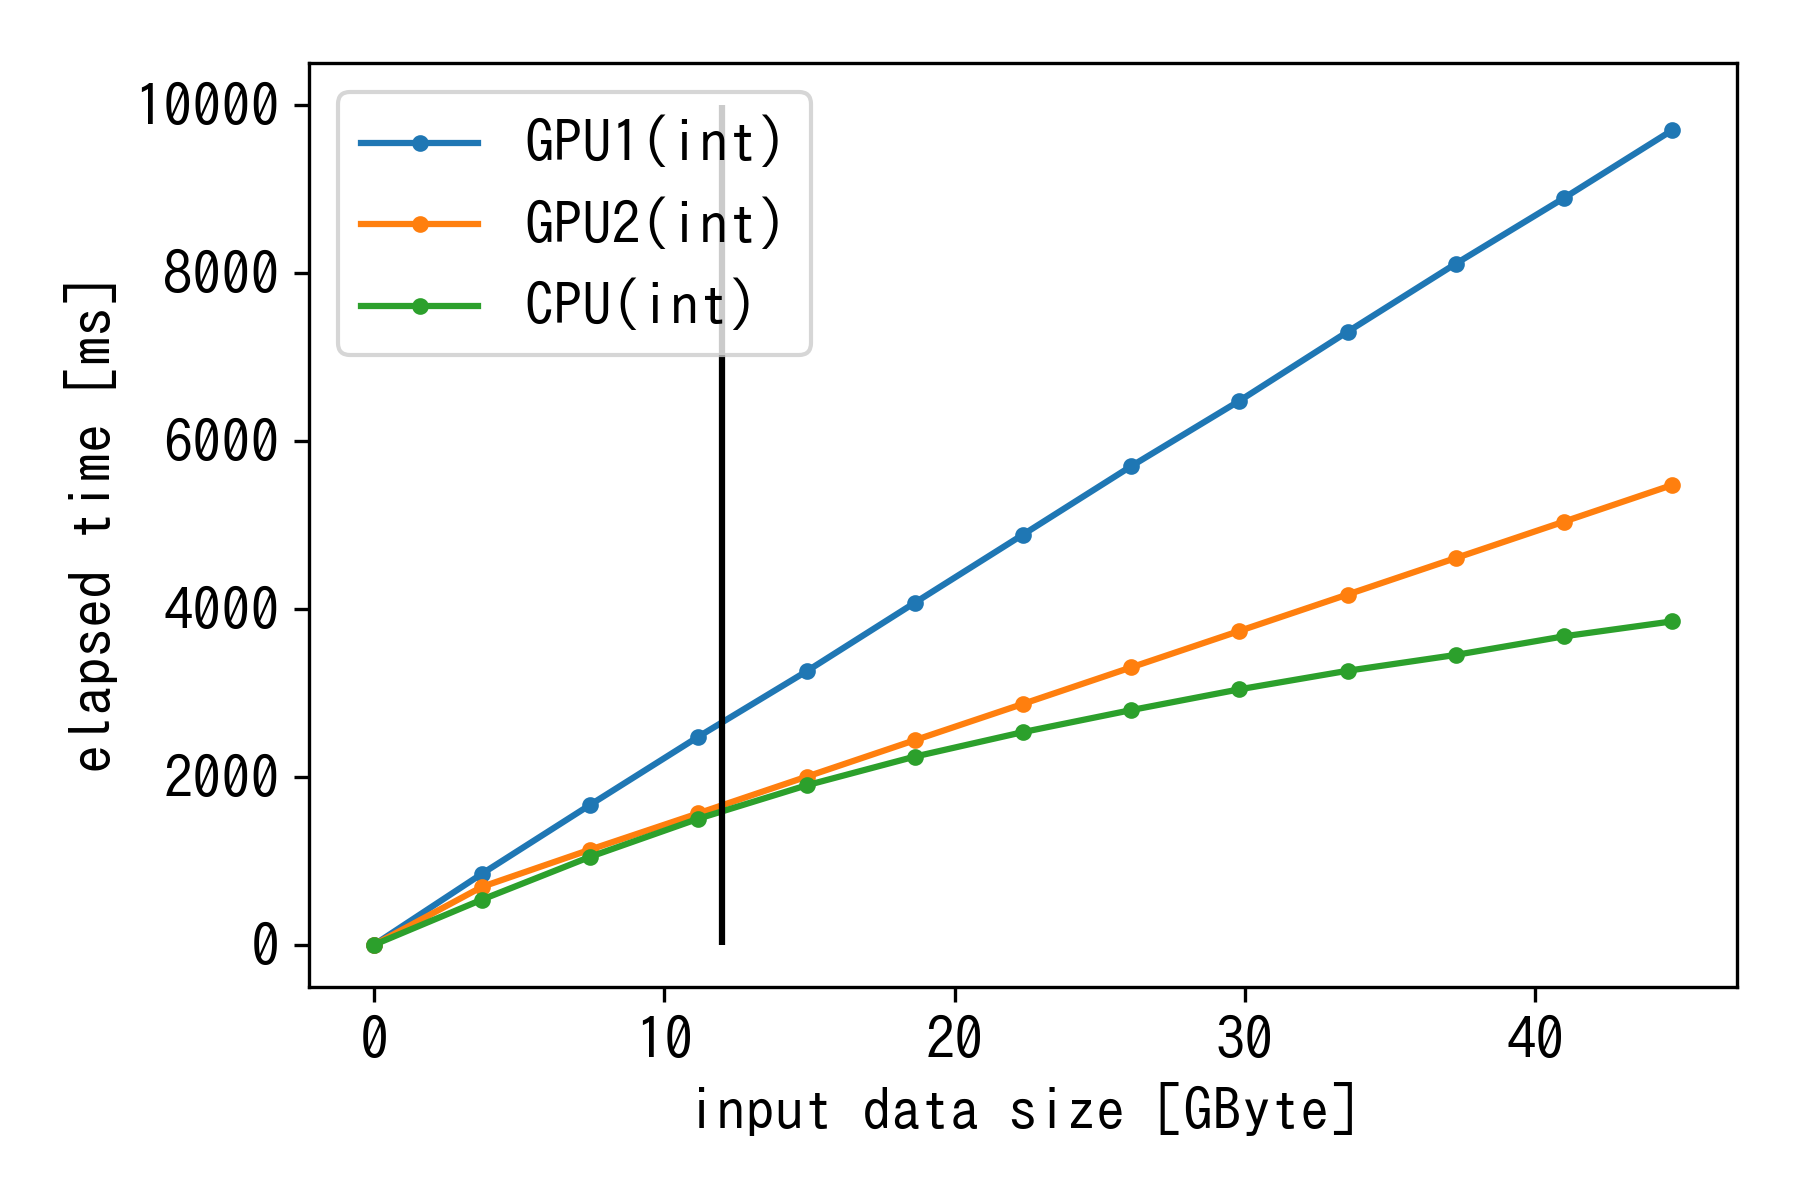
\includegraphics[width=0.8\linewidth]{figures/plt_merge_elapsed2_docker.png}
  \caption{実行時間}
  \label{fig:elapsed}
\end{figure}

\end{document}
